\chapter{Regresión}
\label{sec:reg}
El objetivo principal de esta sección es el de comprobar el comportamiento de una serie de modelos e intentar mejorar el rendimiento de los mismos, añadiendo nuevos pasos a la etapa de pre-procesamiento y volviendo a entrenar los modelos que se han seleccionado. \\
Como se ha comentado previamente, se está trabajando sobre un problema bastante peculiar, donde se intenta predecir distintas variables ordinales. Antes de comenzar con algoritmos más complejos, el primer enfoque para resolver el problema ha sido el de usar una media de cada variable a predecir. \\
Es cierto que usando este enfoque, estamos perdiendo información muy importante: se está suponiendo que todas las variables son igualmente importantes, lo cual es una desventaja de esta aproximación al problema.
Por el contrario, este enfoque tiene la ventaja de estar usando algoritmos clásicos de regresión, proporcionando una salida más general, además de que usando este enfoque primero, descartamos la posibilidad de tener un conjunto de datos con mucho ruido o con un mal muestreo de los datos.

\section{Modelos de regresión}
En esta sección, se va a mostrar los resultados obtenidos por los modelos seleccionados en \ref{sec:algoritmos}-\nameref{sec:algoritmos}.
\subsection{Árboles de decisión}
En esta sección se muestran los resultados obtenidos por el \textbf{Árboles de Decisión}, explicado en la sección \ref{alg:dec_tree}-\nameref{alg:dec_tree}.
\subsubsection*{Procesado de datos}
Antes de ejecutar la fase de entrenamiento, hay que modificar los datos para adaptarlos a las limitaciones del modelo. En este caso, los Árboles de Decisión no admiten valores perdidos y debido a ciertas limitaciones de la librería que se está usando, no son capaces de trabajar con variables categóricas, aunque generalmente si son capaces de trabajar con este tipo de variables..\\
Las modificaciones que se han hecho previamente son: (por orden)
\begin{enumerate}
	\item \textbf{Imputación de valores perdidos}
	\item \textbf{Transformación de variables categóricas a numéricas}
\end{enumerate}
Por este motivo, se ha tenido que introducir una fase extra transformando las variables categóricas en numéricas.
\subsubsection*{Resultados}
\label{sec:res_tree}
Antes de mostrar los resultados, hay que destacar que cuando se entrena un árbol de decisión sin limitar los parámetros, este va a seguir separando los datos de entrenamiento hasta que no pueda realizar más divisiones. Para encontrar el árbol óptimo, primero se ha entrenado el árbol por defecto y se han obtenido los parámetros. Esos parámetros se han establecido como limite, se han entrenado varios árboles con distintos parámetros (sin superar el límite establecido por el primer modelo) y se ha escogido el que mejores resultados obtenía. Los parámetros que mejor resultados dieron son: \\
\begin{itemize}
	\item \textbf{Profundidad máxima:} Limita la profundidad (cantidad de preguntas) del árbol. El mejor valor ha sido \textbf{8}
	\item \textbf{Máximo número de hojas:} Máximo numero de hojas (grupos en el último nivel de una rama). El mejor valor ha sido \textbf{16}
\end{itemize}
En la Tabla \ref{tab:tree_res} se van a exponer los resultados obtenidos usando Árboles de Decisión sobre 5 conjuntos de validación. También se va a mostrar los valores obtenidos a la hora de predecir el propio conjunto de entrenamiento y el conjunto de test.
\begin{table}[H]
	\centering
	\begin{tabular}{|c|c|c|c|c}
		\cline{1-4}
		FOLD   & R2    & Poisson Deviance & MSE   \\ \cline{1-4}
		Fold 0 & 0.678 & 0.211            & 0.886 \\ \cline{1-4}
		Fold 1 & 0.661 & 0.206            & 0.884 \\ \cline{1-4}
		Fold 2 & 0.629 & 0.239            & 0.98  \\ \cline{1-4}
		Fold 3 & 0.67  & 0.191            & 0.8   \\ \cline{1-4}
		Fold 4 & 0.636 & 0.211            & 0.933 \\ \cline{1-4}
		Fold 5 & 0.655 & 0.212            & 0.897 \\ \cline{1-4}
		Train  & 0.748 & 0.156            & 0.659 \\ \cline{1-4}
		Test   & 0.69  & 0.196            & 0.815 \\ \cline{1-4}
	\end{tabular}
	\caption{Árbol de decisión: Profundidad 8, número máximo de hojas 16}
	\label{tab:tree_res}
\end{table}
\pagebreak
A continuación se muestra el gráfico de dispersión de errores:
\begin{figure}[H]
	\centering
	\includegraphics[scale=0.8]{src/scattered_error_DT.png}
	\caption{Gráfico de dispersión de errores}
	\label{fig:tree_scattered}
\end{figure}
En la Figura \ref{fig:tree_scattered} se puede observar que los valores predichos por el Árbol de decisión siguen un patrón muy artificial, apareciendo muchos de ellos juntos y en la misma horizontal. El que estas horizontales aparezcan cerca de un valor concreto, no implica que estas estén bien clasificada.
Con esta información podemos concluir que Árboles de decisión, aunque los resultados no han sido malos teniendo en cuenta que es un algoritmo más simple que el resto, no ha sido capaz de capturar todo el conocimiento que hay en el conjunto ya que no se puede observar la \quotes{dispersión} que aparece en el conjunto de datos real.\\
También se puede apreciar que la mayoría de datos reales aparecen en la parte superior mientras que en la parte inferior se observan menos instancias. Cabe esperar que la cantidad de fallos que cometa el algoritmo en estos rangos sea menor, ya que la cantidad de muestras es menor.\\
\clearpage
Continuando con las gráficas, e continuación se muestra una gráfica con el conteo de errores por clase:
\begin{figure}[H]
	\centering
	\includegraphics[scale=0.8]{src/error_hist_DT.png}
	\caption{Conteo de errores}
	\label{fig:tree_error_plot}
\end{figure}
En la Figura \ref{fig:tree_error_plot} se puede observar que tenemos una menor cantidad de errores en la parte baja de la variable objetivo. También se aprecia como para valores más altos, la tasa de error comienza a subir. \\Esto puede estar causado debido a que la dispersión en valores altos es muy baja (véase la Figura \ref{fig:tree_error_plot}).
Hay que analizar este comportamiento junto con el resto de modelos, para ver si el problema esta causado por los datos (en este caso el comportamiento se debería de repetir) o es causado por el propio modelo.
\clearpage
\subsubsection*{Representación}
Como se mencionó en la sección \textbf{\ref{alg:dec_tree}-\nameref{alg:dec_tree}}, los árboles de decisión tienen la ventaja de que pueden representarse fácilmente. \\
En este caso, vamos a usar una representación gráfica del árbol, las reglas que ha obtenido el árbol y las variables más importantes.\\
A continuación, en la Figura \ref{fig:decission_tree1}, se muestra la representación gráfica del árbol de decisión entrenado:
\begin{figure}[H]
	\includegraphics[scale=0.3]{src/dtree_plot.png}
	\caption{Árbol de decisión}
	\label{fig:decission_tree1}
\end{figure}
Analizando el árbol representado en la Figura \ref{fig:decission_tree1}, se puede observar que para el rendimiento que se ha obtenido, el árbol de salida no es excesivamente complejo y puede ser leído perfectamente por una persona que no tenga unos grandes conocimientos en como funciona el algoritmo, ya que se puede representar gráficamente el resultado obtenido. \\
\linebreak
Las variables variables en los niveles más altos son las que van a aparecer como más importantes (son las que mejor dividen el conjunto de datos) y a medida que se desciende por los niveles del árbol, estas variables cobran menos relevancia. \\
Gracias a esto, podemos representar gráficamente cuales son las variables que más contribuyeron a la hora de formar el modelo.\\
\linebreak
A continuación, en la Figura \ref{fig:feature_dtree}, se muestran un gráfico con las 10 variables que el modelo consideró con más relevancia. El valor asociado a cada variable es la \textbf{importancia Gini}:
\begin{figure}[H]
	\centering
	\includegraphics[scale=0.3]{src/feature_importance_DT}
	\caption{10 variables más importantes según Árboles de Decisión}
	\label{fig:feature_dtree}
\end{figure}
Volviendo a la documentación proporcionada para comprobar el significado de esos valores:
\begin{itemize}
	\item \textbf{AE5:} Pregunta 5 sobre Actitudes financieras empresariales. Valor $0.735667$
	\item \textbf{AcMedia:} Variable global de Actitud emprendedora. Valor $0.156046$
	\item \textbf{SE2:} Estoy preparado para iniciar una empresa viable. Valor $0.037300$
	\item \textbf{SE5:} Conozco cómo desarrollar un proyecto empresarial. Valor $0.014692$
	\item \textbf{NS1:} Mi familia aprobaría el que yo decidiese crear una empresa. Valor $0.012393$
	\item \textbf{Beca:} Tiene beca el encuestado. Valor $0.008256$
	\item \textbf{Nota:} Nota media del expediente académico hasta la fecha de la encuesta sobre 10 puntos. Valor $0.008034$
	\item \textbf{BA3.f:} Esta variable es positiva si se han contestado las opciones \quotes{\textit{en casa, en cuenta de ahorro, darlo a la familia, productos de inversión, de otro modo}} en la pregunta: \quotes{\textit{En los últimos 12 meses, ¿has ahorrado personalmente algún dinero de alguna de las siguientes formas, independientemente de si aún dispones del dinero?}}. Valor $0.007389$
	\item \textbf{CEF19:} Pregunta sobre Conocimientos financieros empresariales. Valor $0.007202$
	\item \textbf{AE7:} Pregunta 7 sobre Actitudes financieras empresariales. Valor $0.006518$
\end{itemize}
De las columnas \textit{AEx} y \textit{CEFx} no hay información en la documentación, unicamente se menciona que son una serie de preguntas relacionadas con actitudes financieras empresariales y sobre conocimientos financieros empresariales respectivamente.
\pagebreak
\subsection{Random Forest}
En esta sección se muestran los resultados obtenidos por el \textbf{Random Forest}, explicado en la sección \ref{alg:rf}-\nameref{alg:rf}.
\subsubsection*{Procesado de datos}
Al igual que los árboles de decisión, se ha hecho una imputación de valores perdidos y se ha transformado las variables categóricas a numéricas debido a limitación que hay en la librería usada.
\subsubsection*{Resultados}
Antes de mostrar los resultados, estos son los parámetros que se han usado al entrenar el modelo:
\begin{itemize}
	\item \textbf{max\_features}: Número de variables que se van a escoger de manera aleatoria: $\frac{1}{3}$ del número de variables.
	\item\textbf{n\_estimators}: Número de árboles que forman el Random Forest: $500$
\end{itemize}
En la Tabla  \ref{tab:res_random_forest}, se puede observar los resultados obtenidos por el modelo Random Forest en los 5 conjuntos de validación. conjunto de entrenamiento y test.
\begin{table}[H]
	\centering
	\begin{tabular}{|c|c|c|c|c}
		\cline{1-4}
		FOLD   & R2    & Poisson Deviance & MSE   \\ \cline{1-4}
		Fold 0 & 0.767 & 0.155            & 0.642 \\ \cline{1-4}
		Fold 1 & 0.775 & 0.137            & 0.586 \\ \cline{1-4}
		Fold 2 & 0.741 & 0.17             & 0.684 \\ \cline{1-4}
		Fold 3 & 0.736 & 0.151            & 0.64  \\ \cline{1-4}
		Fold 4 & 0.747 & 0.15             & 0.649 \\ \cline{1-4}
		Fold 5 & 0.753 & 0.153            & 0.64  \\ \cline{1-4}
		Train  & 0.967 & 0.023            & 0.087 \\ \cline{1-4}
		Test   & 0.769 & 0.149            & 0.606 \\ \cline{1-4}
	\end{tabular}
	\caption{Random Forest}
	\label{tab:res_random_forest}
\end{table}
En la Tabla  \ref{tab:res_random_forest} se aprecia una mejora considerable respecto a los resultados obtenidos por Árboles de Decisión, lo que nos indica que la complejidad extra que se añade en este modelo se ve reflejada en una mejora de la capacidad predictiva de este modelo en este problema.
\clearpage
La siguiente figura muestra el gráfico de dispersión de errores:
\begin{figure}[H]
	\centering
	\includegraphics[scale=0.7]{src/scattered_error_rf.png}
	\caption{Gráfico de dispersión de errores}
	\label{fig:rf_scattered}
\end{figure}
Se puede apreciar como a diferencia de Árboles de decisión (Figura \ref{fig:tree_scattered}) Random Forest si ha sido capaz de detectar esa dispersión que hay en el conjunto real y no se aprecia esas horizontales donde se estaban acumulando los valores predichos, si no que están repartidos por todo el espacio. Este comportamiento también se ve por un incremento considerable en los valores de métricas usados.
\clearpage
Continuando con las gráficas, e continuación se muestra una gráfica con el conteo de errores por clase:
\begin{figure}[H]
	\centering
	\includegraphics[scale=0.7]{src/error_hist_rf.png}
	\caption{Conteo de errores}
	\label{fig:rf_error_plot}
\end{figure}
En la Figura \ref{fig:rf_error_plot}, se puede observar una consistencia mayor en los valores predichos, ya que se sigue observando que la diferencia en los errores cometidos para valores bajos y valores altos es más uniforme. También se observa como Random Forest ha tenido un desempeño ligeramente peor para valores bajos, pero ha mejorado en mucho en los valores altos. El comportamiento que se observó en los resultados de Árboles de decisión se ha repetido también aquí. En este momento se debería de empezar a plantearse la opción de añadir una fase nueva a la fase de preprocesamiento para intentar mejorar este comportamiento.\\
\linebreak
A diferencia de Árboles de decisión, Random Forest es un modelo más complejo en el que es más complicado obtener una representación grafica. Se podrían mostrar todos los árboles que forman el bosque, pero hay que tener en cuenta que si el número de árboles que forman el bosque es muy alto, mostrar un gran número de árboles puede ser complicado. Esto demuestra que ha pesar de tener un modelo que rinde mejor, este es mucho más complejo de representar. 
\clearpage
A pesar de que Random Forest es un modelo más complejo que Árboles de Decisión, se puede obtener las variables más importantes calculando el promedio de la importancia de variables de todos los árboles que forman el bosque.\\
En la Figura \ref{fig:feature_rf} se muestra cuales han sido las 10 variables más importantes que ha obtenido Random Forest:
\begin{figure}[H]
	\centering
	\includegraphics[scale=0.4]{src/feature_importance_rf}
	\caption{10 variables más importantes según Random Forest}
	\label{fig:feature_rf}
\end{figure}
Como se puede apreciar en la Figura \ref{fig:feature_rf}, Random Forest ha encontrado un mayor número de variables. \\
Tiene sentido, ya que si volvemos a \ref{alg:rf}-\nameref{alg:rf} se están entrenando varios árboles con conjuntos de datos distintos, lo que aumenta la probabilidad de obtener árboles distintos que probablemente difieran en la importancia que le dan a cada variable.\\
Aún así, se puede observar como las variables \textbf{AE5} y \textbf{AcMedia} tienen una importancia alta en Random Forest y en Árboles de decisión.\\
\linebreak
Para finalizar, se van a mostrar cual es la pregunta/explicación de estas variables que el modelo ha encontrado importantes.
\begin{itemize}
	\item\textbf{AE5:} Pregunta 5 sobre Actitudes financieras empresariales. Valor = $0.246364$
	\item\textbf{AcMedia:} Variable global de Actitud emprendedora. Valor = $0.220202$
	\item\textbf{AC2:} Ser emprendedor es una salida profesional atractiva para mí. Valor = $0.072907$
	\item\textbf{AC4:}Ser emprendedor supondría una gran satisfacción para mí. Valor = $0.065776$
	\item\textbf{AC3:} Si tuviera la oportunidad y los recursos, me gustaría iniciar una empresa. Valor = $0.041642$
	\item\textbf{SEMedia:} Variable global de Autoeficacia emprendedora. Valor = $0.022872$
	\item\textbf{SE2:} Estoy preparado para iniciar una empresa viable. Valor = $0.019630$
	\item\textbf{AC1:} Ser emprendedor implica más ventajas que desventajas para mí. Valor = $0.019396$
	\item\textbf{NS1:} Mi familia aprobaría el que yo decidiese crear una empresa. Valor = $0.014467$
	\item\textbf{Nota:} Nota media del expediente académico hasta la fecha de la encuesta sobre 10 puntos. Valor = $0.012254$
\end{itemize}

\pagebreak
\subsection{KNN}
En esta sección se muestran los resultados obtenidos por el \textbf{K-Nearest Neighbors}, explicado en la sección \ref{alg:knn}-\nameref{alg:knn}.
\subsubsection*{Procesado de datos}
KNN es un algoritmo que depende de la distancia entre dos muestras, esto implica que si una característica del conjunto de datos que se esta usando tiene un rango \textbf{mayor} que otra, esa característica aportará más al cálculo de la distancia, cuando no necesariamente debe de ser así. Por ese motivo, este algoritmo necesita que el conjunto de datos esté \textbf{normalizado} en el momento de entrenar.\\
\linebreak
Este algoritmo, a parte de necesitar que los datos estén normalizados, no admite valores perdidos ni variables categóricas.
\subsubsection*{Resultados}
Antes de mostrar los resultados, estos son los parámetros que se han usado al entrenar el algoritmo:
\begin{itemize}
	\item \textbf{K:} Número de vecinos: 5
	\item \textbf{Métrica:} Distancia usada: Minkowski con $P=2$ (distancia euclidiana).
\end{itemize}
En la Tabla \ref{tab:knn_res} se muestra el resultado obtenido en los 5 conjuntos de validación, conjunto de entretenimiento y test.
\begin{table}[H]
	\centering
	\begin{tabular}{|c|c|c|c|c}
		\cline{1-4}
		FOLD   & R2    & Poisson Deviance & MSE   \\ \cline{1-4}
		Fold 0 & 0.47  & 0.356            & 1.46  \\  \cline{1-4}
		Fold 1 & 0.407 & 0.378            & 1.545 \\  \cline{1-4}
		Fold 2 & 0.449 & 0.362            & 1.457 \\  \cline{1-4}
		Fold 3 & 0.435 & 0.329            & 1.372 \\  \cline{1-4}
		Fold 4 & 0.467 & 0.321            & 1.367 \\  \cline{1-4}
		Fold 5 & 0.446 & 0.349            & 1.44  \\  \cline{1-4}
		Train  & 0.653 & 0.227            & 0.907 \\ \cline{1-4}
		Test   & 0.527 & 0.301            & 1.242 \\ \cline{1-4}
	\end{tabular}
	\caption{KNN: $K=5$, métrica Minkowski con $P=2$}
	\label{tab:knn_res}
\end{table}
Usando este modelo, se puede observar como el valor de las métricas a sido mucho peor que el observado en los modelos que se han analizado previamente.
\clearpage
La siguiente figura muestra el gráfico de dispersión de errores:
\begin{figure}[H]
	\centering
	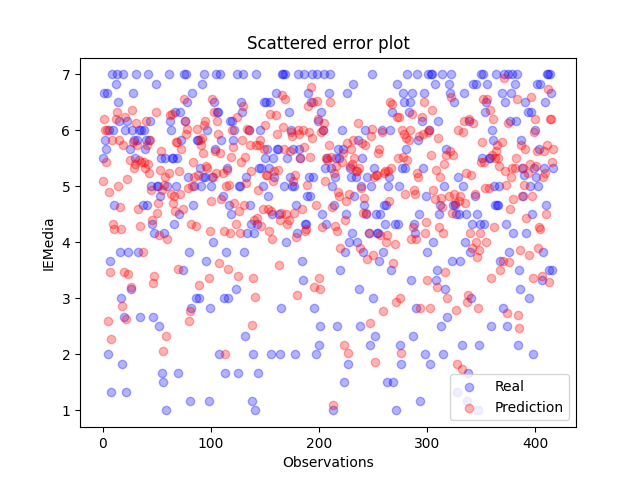
\includegraphics[scale=0.8]{src/scattered_error_knn.png}
	\caption{Gráfico de dispersión de errores}
	\label{fig:knn_scattered}
\end{figure}
Si observamos la Figura \ref{tab:knn_res}, se puede observar como la mayor parte de las predicciones aparecen en la parte central, justo donde se localizan la mayor parte de valores reales. Una posible explicación de este comportamiento puede ser debido a que KNN es un modelo que se basa en la distancia que hay entre dos muestras, puede ocurrir que haya la distancia a la zona donde esta localizada la mayor parte sea menor que la distancia al valor real.
\clearpage
A continuación se muestra una gráfica con el conteo de errores por clase:
\begin{figure}[H]
	\centering
	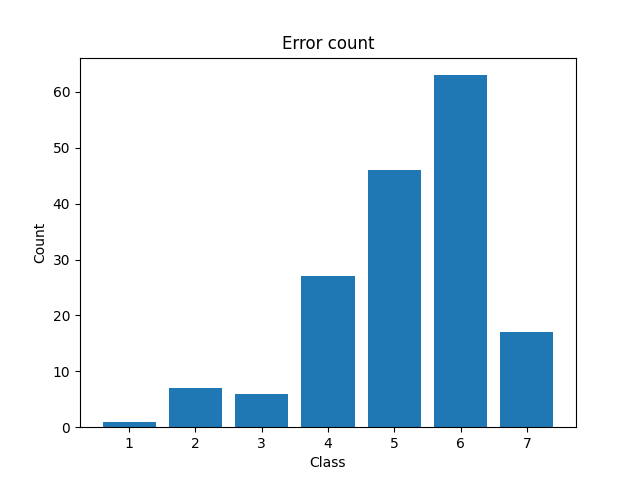
\includegraphics[scale=0.8]{src/error_hist_knn.png}
	\caption{Conteo de errores}
	\label{fig:knn_error_plot}
\end{figure}
Analizando los resultados expuestos en la Figura \ref{fig:knn_error_plot}, se sigue observando el comportamiento explicado en secciones anteriores. Se aprecia como en valores altos, el modelo sigue teniendo una cantidad de errores más o menos igual que el resto de algoritmos mientras que en valores bajos, estos errores son menores.
\clearpage
\subsection{SVM}
En esta sección se muestran los resultados obtenidos por el \textbf{Support Vector Machines}, explicado en la sección \ref{alg:svm}-\nameref{alg:svm}.
\subsubsection*{Procesado de datos}
SVM son modelos con una fuerte base matemática, por lo que son modelos que no pueden ser entrenados usando variables categóricas.
Las modificaciones que se han hecho previamente son: (por orden)
\begin{enumerate}
	\item \textbf{Imputación de valores perdidos.}
	\item \textbf{Escalado de valores numéricos.}
	\item \textbf{Transformación de variables categóricas a numéricas.}
\end{enumerate}
\subsubsection*{Resultados}
A continuación se muestra una tabla con los resultados obtenidos por SVM en el conjunto de validación y en el conjunto de test:
\begin{table}[H]
	\centering
	\begin{tabular}{|c|c|c|c|c}
		\cline{1-4}
		FOLD   & R2    & Poisson Deviance & MSE   \\ \cline{1-4}
		Fold 0 & 0.671 & 0.236            & 0.906 \\ \cline{1-4}
		Fold 1 & 0.718 & 0.186            & 0.734 \\ \cline{1-4}
		Fold 2 & 0.728 & 0.185            & 0.72  \\ \cline{1-4}
		Fold 3 & 0.691 & 0.192            & 0.75  \\ \cline{1-4}
		Fold 4 & 0.697 & 0.193            & 0.776 \\ \cline{1-4}
		Fold 5 & 0.701 & 0.198            & 0.777 \\ \cline{1-4}
		Train  & 0.894 & 0.076            & 0.276 \\ \cline{1-4}
		Test   & 0.737 & 0.173            & 0.691 \\ \cline{1-4}
	\end{tabular}
	\caption{SVM: Tolerancia $1^{-3}$, Kernel RBF, $C=1$}
	\label{tab:svm_res}
\end{table}
En la Tabla \ref{tab:svm_res} se puede observar como este modelo ha obtenido resultados mejores que KNN y Árboles de Decisión, pero SVM no ha llegado a igualar el rendimiento obtenido por Random Forest.
\clearpage
La siguiente figura muestra el gráfico de dispersión de errores:
\begin{figure}[H]
	\centering
	\includegraphics[scale=0.8]{src/scattered_error_svr.png}
	\caption{Gráfico de dispersión de errores}
	\label{fig:svr_scattered}
\end{figure}
En la Figura \ref{fig:svr_scattered} se puede observar como SVM, al igual que Random Forest, ha logrado modelar la dispersión de los datos y no se observan esas predicciones tan artificiales que se observaron en Árboles de Decisión.\\
Se puede observar también como una gran cantidad de predicciones se concentran entre los valores 5 y 6, pero este comportamiento también se puede observar en el resto de modelos.
\clearpage
Finalizando con las gráficas obtenidas para el modelo SVM, a continuación se muestra el conteo de errores.
\begin{figure}[H]
	\centering
	\includegraphics[scale=0.8]{src/error_hist_svr.png}
	\caption{Conteo de errores}
	\label{fig:svr_error_plot}
\end{figure}
Observando la Figura \ref{fig:svr_error_plot}, se vuelve a observar el mismo comportamiento que se ha visto en secciones anteriores, donde en rangos altos los algoritmos están teniendo problemas para predecir estos valores mientras que en valores más bajos no. Definitivamente, se puede confirmar la necesidad de realizar un tratamiento a los datos para intentar mejorar el rendimiento de los modelos seleccionados.
\clearpage
\subsection{XGBoost}
En esta sección se muestran los resultados obtenidos por el \textbf{Xtreme Gradient Boosting}, explicado en la sección \ref{alg:xgb}-\nameref{alg:xgb}.
\subsubsection*{Procesado de datos}
El pre-procesado aplicado para este modelo ha sido similar al usado en Árboles de Decisión:
\begin{enumerate}
	\item \textbf{Imputación de valores perdidos}
	\item \textbf{Transformación de variables categóricas a numéricas}
\end{enumerate}
\subsubsection*{Resultados}
A continuación se muestra una tabla con los resultados obtenidos por \textbf{XGBoost} en los conjuntos de validación, train y test:
\begin{table}[H]
	\centering
	\begin{tabular}{|c|c|c|c|c|}
		\cline{1-4}
		FOLD   & R2    & Poisson Deviance & MSE   \\ \cline{1-4}
		Fold 0 & 0.726 & 0.186            & 0.754 \\ \cline{1-4}
		Fold 1 & 0.734 & 0.165            & 0.693 \\ \cline{1-4}
		Fold 2 & 0.71  & 0.196            & 0.766 \\ \cline{1-4}
		Fold 3 & 0.723 & 0.16             & 0.671 \\ \cline{1-4}
		Fold 4 & 0.744 & 0.157            & 0.658 \\ \cline{1-4}
		Fold 5 & 0.727 & 0.173            & 0.708 \\ \cline{1-4}
		Train  & 0.991 & 0.005            & 0.024 \\ \cline{1-4}
		Test   & 0.741 & 0.162            & 0.68  \\ \cline{1-4}
	\end{tabular}
	\caption{Métricas de XGBoost formado por un total de 30 qqárboles}
	\label{tab:xgboost}
\end{table}
Observando los resultados expuestos en la Tabla \ref{tab:xgboost}, se puede apreciar como XGBoost ha conseguido unos resultados mejores que SVM, Árboles de Decisión y KNN, pero no ha conseguido igualar el rendimiento tan bueno que ha obtenido Random Forest a la hora de resolver este problema.
\clearpage
La siguiente figura muestra el gráfico de dispersión de errores:
\begin{figure}[H]
	\centering
	\includegraphics[scale=0.8]{src/scattered_error_xgboost.png}
	\caption{Gráfico de dispersión de errores para XGBoost}
	\label{fig:xgboost_scattered}
\end{figure}
Al igual que los resultados obtenidos por Random Forest, en la Figura \ref{fig:xgboost_scattered} se puede observar como el rendimiento del modelo ha sido bastante bueno, logrando capturar también esa dispersión que modelos más simples como Árboles de decisión no fueron capaces de modelar.
\clearpage
Finalizando con las gráficas, a continuación se muestra una gráfica con el conteo de errores por clase:
\begin{figure}[H]
	\centering
	\includegraphics[scale=0.8]{src/error_hist_xgboost.png}
	\caption{Conteo de errores}
	\label{fig:xgboost_error_plot}
\end{figure}
En la Figura \ref{fig:xgboost_error_plot} se puede observar el mismo comportamiento que en resto de modelos que se han estudiado en secciones anteriores. Está bastante clara la necesidad de realizar un paso extra en la parte de preprocesamiento para intentar reducir la cantidad de errores que se están cometiendo en los valores más altos.
\clearpage
\subsection{Perceptrón multi-capa}
En esta sección se muestran los resultados obtenidos por el \textbf{Perceptron multicapa}, explicado en la sección \ref{alg:mlp}-\nameref{alg:mlp}.
\subsubsection*{Procesado de datos}
MLP es un algoritmo que no es capaz de ser entrenados usando variables categóricas. Las modificaciones que se han hecho sobre el conjunto de datos son las siguientes:
\begin{enumerate}
	\item \textbf{Imputación de valores perdidos.}
	\item \textbf{Escalado de valores numéricos.}
	\item \textbf{Transformación de variables categóricas a numéricas.}
\end{enumerate}
\subsubsection*{Resultados}
En esta sección se va a mostrar los resultados obtenidos por el Perceptrón Multi-capa. \\
\linebreak
En esta tabla, se puede observar el rendimiento del modelo en los conjuntos de validación, entrenamiento y test:
\begin{table}[H]
	\centering
	\begin{tabular}{|c|c|c|c|c}
		\cline{1-4}
		FOLD   & R2    & Poisson Deviance & MSE   \\\cline{1-4}
		Fold 0 & 0.557 & 0.321            & 1.221 \\\cline{1-4}
		Fold 1 & 0.566 & 0.274            & 1.13  \\\cline{1-4}
		Fold 2 & 0.586 & 0.269            & 1.096 \\\cline{1-4}
		Fold 3 & 0.412 & 0.291            & 1.427 \\\cline{1-4}
		Fold 4 & 0.488 & 0.303            & 1.313 \\\cline{1-4}
		Fold 5 & 0.522 & 0.292            & 1.237 \\\cline{1-4}
		Train  & 0.999 & 0.0              & 0.002 \\\cline{1-4}
		Test   & 0.616 & 0.27             & 1.007 \\\cline{1-4}
	\end{tabular}
	\caption{Perceptrón Multicapa: 1 capa oculta con 100 neuronas con un máximo de 500 iteraciones}
	\label{tab:mlp_res}
\end{table}
Analizando los resultados mostrados en la Tabla \ref{tab:mlp_res}, se puede observar un rendimiento muy pobre debido a un sobre-aprendizaje muy claro. Se observa como en el conjunto de entrenamiento se ha conseguido un muy buen rendimiento, pero a costa de que la red haya aprendido todo el ruido presente en el conjunto de datos.\\
\linebreak
Cabe destacar que este conjunto de datos no parece muy adecuado para hacer uso de este modelo, ya que existe una cantidad alta de variables categóricas, que complican mucho el proceso de entrenamiento usando este modelo.
\clearpage
La siguiente figura muestra el gráfico de dispersión de errores:
\begin{figure}[H]
	\centering
	\includegraphics[scale=0.8]{src/scattered_error_MLP.png}
	\caption{Gráfico de dispersión de errores}
	\label{fig:mlp_scattered}
\end{figure}
En la Figura \ref{fig:mlp_scattered} se puede observar un comportamiento que no se ha observado con el resto de modelos: El modelo entrenado esta prediciendo valores fuera del rango. Este comportamiento se puede explicar debido a que el modelo ha aprendido el ruido del conjunto de datos, sufriendo así de un sobre-aprendizaje. Observando las métricas se puede ver como en el conjunto de entrenamiento el resultado ha sido muy bueno, pero en el conjunto de test no. Este comportamiento también se repite en los conjuntos de validación.
\clearpage
Continuando con las gráficas, e continuación se muestra una gráfica con el conteo de errores por clase:
\begin{figure}[H]
	\centering	\includegraphics[scale=0.8]{src/error_hist_MLP.png}
	\caption{Conteo de errores}
	\label{fig:mlp_error_plot}
\end{figure}
Aunque el rendimiento de este modelo ha sido el peor, analizando los resultados de la Figura \ref{fig:mlp_error_plot}, se sigue observando el mismo comportamiento que en los modelos previos, evidenciando una vez más la necesidad de ese procesamiento extra que es necesario para intentar mejorar los resultados.
\clearpage
\section{Análisis de resultados}
Se ha observado que los modelos basados en Árboles de Decisión y Random Forest han tenido un buen comportamiento, por lo que se ha optado por seguir haciendo uso de ellos en secciones siguientes. XGBoost, tiene unos resultados ligeramente peores respecto a Random Forest pero con un comportamiento similar, fallando considerable en valores altos de intención emprendedora media). Como XGBoost no esta aportando nada nuevo, por ahora se va a descartar.\\
\linebreak
SVR se ha comportado casi al nivel de modelos como XGBoost o Random Forest. Por ahora, no se va a descartar su uso, ya que introduciendo el conocimiento que se ha obtenido usando modelos como Random Forest o árboles de decisión se podría mejorar el rendimiento.\\
\linebreak
Los resultados obtenidos por  KNN demuestran que este algoritmo no funciona bien con el conjunto de datos que se está usando. La razón más probable por la que KNN obtuvo estos resultados, es que hay relaciones entre las variables que KNN no es capaz de detectar, al comparar únicamente la distancia característica por característica. Debido al bajo desempeño que se ha obtenido al usar KNN, va a ser descartado de las siguientes fases.\\
\linebreak
Respecto al Perceptrón Multicapa, ya que el rendimiento en comparación con otros modelos probados y debido al enorme coste de entrenamiento que pueden llegar a tener, se ha decidido no continuar haciendo uso de este modelo.\\
\linebreak
Como ya se ha mencionado, los modelos basados en árboles de decisión son capaces de obtener la importancia de las características. A continuación se muestran una gráfica recogiendo los valores de importancia de variables para facilitar la comparación:
\begin{figure}[H]
	\centering
	\includegraphics[scale=0.7]{src/rf_dt_features}
	\caption{Variables más importantes según Random Forest y Árboles de Decisión}
	\label{fig:feature_rf2}
\end{figure}
Como se ve en las Figura \ref{fig:feature_rf2}, vemos que hay dos variables que \textbf{ambos} algoritmos han dado como más importantes:
\begin{itemize}
	\item\textbf{AE5:} Pregunta  5 sobre Actitudes financieras empresariales.
	\item\textbf{AcMedia:} Variable global de Actitud emprendedora.
\end{itemize}
También se puede observar como Random Forest ha encontrado importantes variables que Árboles de Decisión no ha marcado como importantes. Esto demuestra otra vez que Random Forest es un modelo mucho más robusto que Árboles de Decisión y que es capaz de extraer más conocimiento del conjunto de datos con el que se está trabajando.\\
\linebreak
Repasando los resultados, se puede apreciar que a todos los algoritmos usados les está costando predecir correctamente los valores altos para la intención emprendedora media (véase Figura \ref{fig:rf_error_plot}). Este comportamiento ha sido constante para cada algoritmo usado. La causa de este comportamiento puede ser que a medida que se incrementa el valor de intención emprendedora media, los datos son menos dispersos y a los algoritmos les está costando distinguir entre varios valores cercanos. Este comportamiento se puede apreciar en los gráficos de dispersión de errores que se han mostrado previamente.
\pagebreak
\section{Muestreo de datos}
Una vez se ha comprobado el rendimiento de los distintos modelos que se han seleccionado, se va a intentar mejorarlo añadiendo nuevas etapas extra al procesamiento de datos antes de entrenar los modelos.
\newline
Como se ha podido observar en la primera iteración, todos los algoritmos se están equivocando en valores altos. Para intentar reducir el ruido, se va tratar el conjunto de datos haciendo \textbf{under-sampling}.\\
Under-Sampling (se podría traducir como \textit{muestreo}) es una técnica para reducir el ruido del conjunto de datos eliminando algunas muestras del conjunto de datos.\\
\linebreak
Como se puede ver en la \ref{tab:ocurrencia_valores} donde se muestra la ocurrencia de valores para las distintas variables a predecir,  aquellos con un valor alto son los más predominantes, siendo en estos valores donde los algoritmos más se están equivocando. El motivo puede ser que al estar prediciendo la media de las distintas variables, se está introduciendo una gran cantidad de ruido. \\
En valores bajos, como se puede ver en la Figura \ref{fig:rf_error_plot} donde se muestra el gráfico de errores para Random Forest, la cantidad de fallos en el algoritmo para estos valores es mucho menor. Esta tendencia se repite en todos los algoritmos.\\
\subsection{Algoritmo}
Para realizar el proceso de muestreo, se ha desarrollado el siguiente algoritmo:
\begin{enumerate}
	\item Se entrena un modelo de aprendizaje con el conjunto de entrenamiento.
	\item Por cada muestra del conjunto de entrenamiento, se predice el valor usando el modelo entrenado.
	\item Se comprueba la diferencia entre valor real y el valor predicho.
	\item Si la diferencia es mayor que un umbral, se elimina esa muestra del conjunto de entrenamiento.
\end{enumerate}
El modelo entrenado para hacer muestreo, es un árbol de decisión con un máximo de $4$ niveles, eliminando muestras de todo el rango de predicción.\\
\linebreak
Con este algoritmo, vamos a ver que impacto tiene el eliminar estas muestras ruidosas. En el mejor de los casos, deberíamos observar un incremento en los valores de las métricas que se han usado. En el peor de los casos, puede ocurrir que al eliminar estas muestras, perdamos información y que el rendimiento de los modelos sea peor.
\clearpage
\subsection{Resultados}
A continuación se muestra una serie de gráficos comparando los resultados obtenidos por los algoritmos seleccionados.\\
\linebreak
Con el objetivo de ajustar lo mejor posible los parámetros que se están usando para el algoritmo explicado en la sección anterior, se ha optado por elegir distintos umbrales dentro del rango $\left[0.4,1\right)$, mostrando de forma gráfica una comparativa con las métricas obtenidas con los distintos umbrales.\\
Los valores que se aprecian en las leyendas de las figuras equivalen al valor del umbral para el que se ha obtenido ese valor.\\
\linebreak
En los párrafos siguientes, se van a mostrar los resultados obtenidos por los modelos que han sido seleccionados: Árboles de Decisión, Random Forest y Máquinas de Soporte de Vectores.
\subsubsection*{Árboles de Decisión}
La gráfica que se muestra a continuación compara el rendimiento medio en el conjunto de validación.
\begin{figure}[H]
	\centering
	\includegraphics[scale=0.8]{src/dtree_undersamp_val_metrics.png}
	\caption{Media en validación usando under-sampling}
	\label{fig:cmp_val_dtree}
\end{figure}
Respecto a las métricas obtenidas en los conjuntos de validación mostradas en la Figura \ref{fig:cmp_val_dtree}, se puede apreciar que en cuanto al valor obtenido por $R2$ se ha mantenido, pero se ha mejorado drásticamente el valor en las métricas \textit{Desviación de Poisson} y \textit{MSE}. Esto indica que el modelo obtenido tras el procesamiento se ajusta mejor a los datos.\\
\linebreak
Continuando con las gráficas comparativas, se va a mostrar una gráfica comparando las métricas obtenidas en el conjunto de test.
\begin{figure}[H]
	\centering
	\includegraphics[scale=0.8]{src/dtree_undersamp_test_metrics.png}
	\caption{Métricas en test usando under-sampling}
	\label{fig:cmp_test_dtree}
\end{figure}
Como se puede ver en la Figura \ref{fig:cmp_test_dtree}, las métricas en test son ligeramente mejores tras reducir el ruido dentro del conjunto de entrenamiento.\\
Los mejores resultados se han obtenido usando el muestreo de la forma más agresiva, tomando como umbral el valor $0.5$ y eliminando un total de $628$ muestras.
\clearpage
Finalmente, se va a mostrar el gráfico de comparación de errores cometidos.
\begin{figure}[H]
	\centering
	\includegraphics[scale=0.8]{src/dtree_undersamp_error_hist.png }
	\caption{Comparación de errores usando under-sampling}
	\label{fig:cmp_error_dtree}
\end{figure}
Como se aprecia en la Figura \ref{fig:cmp_error_dtree}, usando el algoritmo de muestreo, se ha reducido la cantidad ruido en los rangos más altos de predicción, mejorando así el rendimiento del árbol de decisión para estos valores y estabilizando las zonas donde se estaba comportando peor.\\
\linebreak
También se puede observar como se ha incrementado por mucho el valor de errores entorno al valor $4$, pero no ha influido negativamente en los valores de las métricas. Hay que recordar que esta tabla es una \textbf{aproximación} y que las métricas usadas tienen en cuenta muchos más factores importantes.\\
\linebreak
En general, se aprecia una mejora en árboles de decisión reduciendo el ruido del conjunto de datos, ya que los árboles de decisión son algoritmos bastantes sensibles al ruido.
\clearpage
\subsubsection*{Random Forest}
Para finalizar, a continuación se va a mostrar los resultados obtenidos por Random Forest en el conjunto de validación.
\begin{figure}[H]
	\centering
	\includegraphics[scale=0.8]{src/rf_undersamp_val_metrics.png}
	\caption{Media en validación usando under-sampling}
	\label{fig:cmp_val_rf}
\end{figure}
Analizando los resultados mostrados en la Figura \ref{fig:cmp_val_rf}, donde se muestra el rendimiento en el conjunto de validación, se puede apreciar como a medida que se reduce la cantidad de muestras eliminadas, los valores tienden a ser peores. Como se ha visto en la sección anterior, esta mejora en validación puede no implicar una mejora en los valores obtenidos en test, por lo que antes de valorar si hay mejora o no, hay que observar los valores obtenidos en test.\\
\clearpage
A continuación se muestran los resultados obtenidos en el conjunto de test.
\begin{figure}[H]
	\centering
	\includegraphics[scale=0.8]{src/rf_undersamp_test_metrics.png}
	\caption{Métricas en test usando under-sampling}
	\label{fig:cmp_test_rf}
\end{figure}
En la Figura \ref{fig:cmp_test_rf}, donde se muestra el rendimiento en el conjunto de test, se puede apreciar como Random Forest ha obtenido los mejores resultados se han obtenido usando el conjunto de datos original.\\
\linebreak
También se puede apreciar como usando umbrales entre $\left[0.5,0.9\right]$ no se ha observado un cambio relevante en los métricas. Esta mejora solo se ha observado usando umbrales muy altos, donde se han eliminado la menor cantidad de muestras.\\
\linebreak
Esto demuestra que para modelos que Random Forest es un modelo mucho más robusto frente al ruido que Árboles de Decisión, donde se pudo apreciar la mejora en el rendimiento en el momento que se eliminaron ciertas muestras del conjunto de entrenamiento.
\clearpage
Para finalizar mostrando los resultados obtenidos por Random Forest, se va a mostrar la gráfica de errores cometidos por rango.
\begin{figure}[H]
	\centering
	\includegraphics[scale=0.8]{src/rf_undersamp_error_hist.png }
	\caption{Comparación de errores usando under-sampling}
	\label{fig:cmp_error_rf}
\end{figure}
En la Figura \ref{fig:cmp_error_rf} se puede apreciar una mejora para los rangos más altos de Intención Emprendedora. Esta mejora también se aprecia en los rangos más bajos. \\
Donde si que no se observa una mejora, o incluso se empeora los resultados, es en las zonas medias, donde el valor más bajo de errores se ha obtenido usando el conjunto de datos original.
\clearpage
\subsubsection*{SVR}
Continuando con los modelos seleccionados, a continuación se muestran los resultados obtenidos usando Máquinas de Soporte de Vectores.\\
\linebreak
Para empezar analizando los resultados, se va a mostrar los valores obtenidos en el conjunto de validación.
\begin{figure}[H]
	\centering
	\includegraphics[scale=0.8]{src/svr_undersamp_val_metrics.png}
	\caption{Media en validación usando under-sampling}
	\label{fig:cmp_val_svr}
\end{figure}
En la Figura \ref{fig:cmp_val_svr} se puede observar como en validación, SVM parece que ha mejorado ligeramente el rendimiento cuando se han eliminado esas muestras más ruidosas, por lo que es una indicación de que el modelo sigue siendo bueno a la hora de extraer el conocimiento del conjunto de datos.\\
\clearpage
Continuando con el análisis de resultados, se van a mostrar los valores obtenidos en el conjunto de test.
\begin{figure}[H]
	\centering
	\includegraphics[scale=0.8]{src/svr_undersamp_test_metrics.png}
	\caption{Métricas en test usando under-sampling}
	\label{fig:cmp_test_svr}
\end{figure}
Analizando los resultados expuestos en la Figura \ref{fig:cmp_test_svr}, SVM parece que no se ha visto tan beneficiado a la hora de eliminar estas muestras más ruidosas. Se puede observar como la cantidad de errores cometidos (en amarillo) es menor que en el resto de modelos entrenados.\\
Como se explicó en la Sección \nameref{alg:dec_tree}, los Árboles de Decisión son modelos que son muy sensibles al ruido, por lo que es de esperar que la mejora observada a la hora de eliminar estas muestras sea mayor que en modelos más robustos como SVM.\\
\clearpage
Para finalizar, se va a mostrar la gráfica de errores cometidos por el modelo
\begin{figure}[H]
	\centering
	\includegraphics[scale=0.8]{src/svr_undersamp_error_hist.png }
	\caption{Comparación de errores usando under-sampling}
	\label{fig:cmp_error_svr}
\end{figure}
Se puede apreciar como esa bajada de rendimiento que se observó en la Figura \ref{fig:cmp_test_svr} se observa también en la Figura \ref{fig:cmp_error_svr}, donde la cantidad de errores cometidos es menor en los casos donde no se han eliminado muestras, incrementando la tasa de errores especialmente en valores altos.\\
\linebreak
Debido a que este modelo es mucho más robusto que Árboles de Decisión, la mejora observada no se ha aplicado a la hora de hacer uso de este modelo.\\
Parece que el hiper-plano que encontró el modelo con el conjunto de datos completo se adapta mejor al conjunto de test.
\clearpage
\subsection{Análisis de resultados}
Se ha apreciado una mejora en en los algoritmos basados en árboles de decisión. La principal mejora ha sido el obtener una menor cantidad de errores en aquellas zonas donde los algoritmos se están comportando peor. También se ha podido observar que Random Forest obtuvo mejores resultados con un umbral más alto que Árboles de Decisión. \\
La causa más probable de que necesite un umbral más alto es que al usar varios árboles para predecir el resultado, la probabilidad de que varios árboles contradigan el valor predicho por un árbol que clasificó mal un valor es alta. Por eso, al eliminar aquellas muestras más problemáticas del conjunto, el propio Random Forest es capaz de lidiar con el ruido de muestras que son menos problemáticas y beneficiarse de tener un conjunto de entrenamiento más grande.\\
\linebreak
Respecto a SVM, observando los resultados obtenidos, se aprecia que ha medida que se reduce la cantidad de muestras que se eliminan, el rendimiento es mejor.
Como se están eliminando muestras que pueden estar en la frontera (o incluso vectores soporte), es posible que el hiper-plano calculado por el modelo de un menor margen o sea en general peor.\\
\linebreak
Como el único cambio que se ha observado ha sido en Árboles de Decisión, se va a comparar la importancia de variables obtenida en el conjunto original y en el conjunto en el que se han eliminado las muestras más ruidosas.\\
\clearpage
A continuación, en la Figura \ref{fig:cmp_fi_dt} se va a mostrar una gráfica con la comparativa entre el modelo entrenado en el conjunto de datos original y en el conjunto de datos muestreado.
\begin{figure}[H]
	\centering
	\includegraphics[scale=0.7]{src/dt_dt_und_features}
	\caption{Comparación de importancia de variables}
	\label{fig:cmp_fi_dt}
\end{figure}
Se puede apreciar en la Figura \ref{fig:cmp_fi_dt}, las variables más importantes a la hora de realizar la predicción siguen presentes, pero la variable \textbf{AE5} es ligeramente menos importante una vez que se han eliminado las muestras más ruidosas. En cambio, para la variable \textbf{ACMedia}, se puede observar el comportamiento contrario, un incremento en la importancia de esta variable. \\
\linebreak
También se aprecia como, para variables que no han influido tanto en la predicción usando el conjunto de datos original, se ha reducido la influencia de las mismas, llegando incluso a tener muy poca o ninguna relevancia en el conjunto de datos muestreado.
